\section{Are there Grandmother Cells in CNNs? How distributed are the representations?}
\label{sec:grand-mother}
Neuroscientists have conjectured that cells in the human brain which only respond to very specific and complex visual stimulus (such as the face of one's grandmother) are involved in object recognition and termed them as Grandmother Cells (GMC) \cite{Barlow}, \cite{Grandmother}. Proponents of artificial neural networks have shown a great interest in reporting the presence of GMC like filters for specific object classes in their networks \cite{GoogleCat}. More recently, for understanding feature representations in CNN, \cite{DeConv}, \cite{Simonyan} presented methods for finding the optimal visual input for individual filters. Mathematically, this computation is expressed as finding the set of images $\mathcal{I}$ which maximally activate a single feature (i.e. find $i \in \mathcal{I}$ s.t. Feature-score(i) $\geq th$ $\forall i $, where $th$ is a threshold value). The distribution of class labels associated with this set of images ($\mathcal{I}$), defines the \textit{precision} of the feature. However, this distribution does not account for the \textit{recall}.  The presence/absence of GMC is a scientifically interesting question to pursue, but for recognition, we require features with both high precision and high recall. Consequently, we argue that if the goal is object recognition, then GMC for a particular object class should be interpreted as features with high AP and not just high precision. 
 
Further, prior to the work of \cite{Kriz}, the dominant approaches for image and scene classification were based on either representing images as a bag of local descriptors (or words) such as SIFT (BoW model, \cite{SPM}) or using mid-level patches \cite{Mid1}, \cite{Blocks}. The BoW feature representation is a distributed code (i.e. a single feature by itself is not discriminative, but a group of features taken together is.), whereas the problem of finding good mid-level patches is often posed as a greedy search for high recall discriminative templates. Mid-level patches are closer to the GMC-like representation. Given this, it is interesting to investigate the CNN features to find the kind of representations they employ.

We perform such analysis in two phases using conv-5 features. In the first phase, we directly address the question of finding GMC (section \ref{sub:class-specific-unit}) by computing AP of individual filters. Next, we determine the total number of filters required for achieving the same performance as all the filters for objectively assessing how distributed are the feature representations (section \ref{sub:how-many}).

\subsection{Finding Grandmother Cells}
\label{sub:class-specific-unit}
%Precision for each filter from layer 5 is computed in a way analogous to entropy computation described in \ref{sub:def-ent}. In the final step instead of computing the entropy, we compute Prob(Class $|$ Filter Activity $\geq$ threshold). We define the selectivity of a filter as the area under the precision curve. 

%For this computation we use ground truth bounding boxes taken from PASCAL VOC-2007 test challenge.
%From figure \ref{fig:ap} it is clear that for some classes such persons and bicycles there are indeed some very high precision filters, but for a lot of classes like sofa and horses no such filters exist. 

\begin{figure}[t!]
\centering
\subfloat{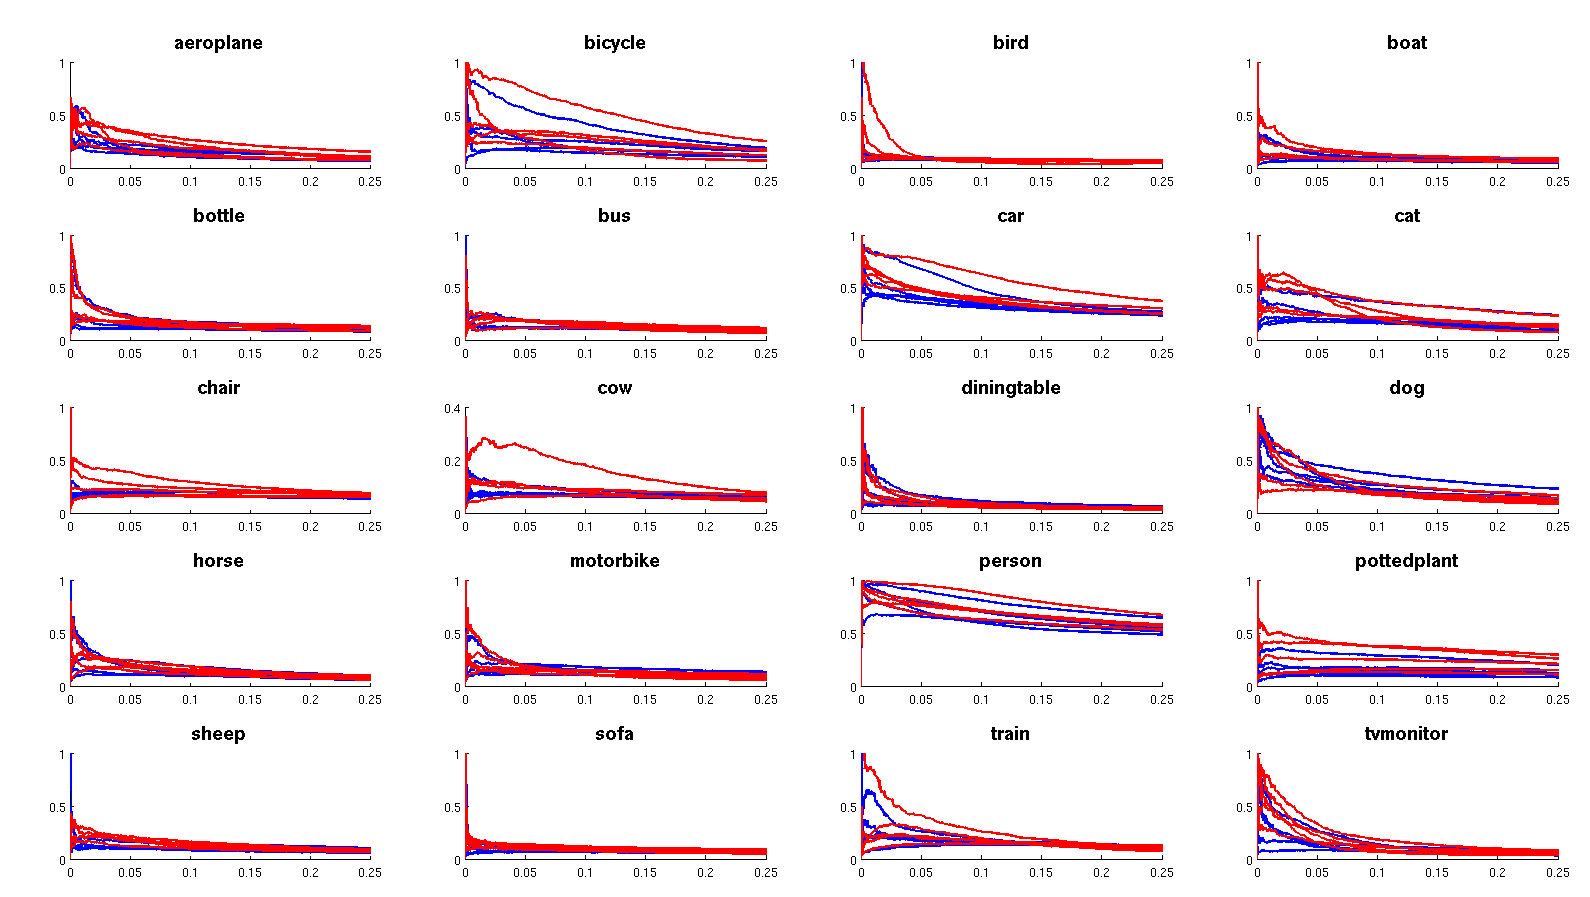
\includegraphics[scale=0.20]{images/gtbbox_pascal_prerec_pool5units.png}}
\caption{The precision-recall curves for the top five (based on AP) conv-5 filter responses on PASCAL-DET-GT. Red-Curves: Fine Tuned Network, Blue-Curves: Pre-Trained Network. For most classes, precision drops significantly even at modest recall values. \todo{update figure with PDF}}
\label{fig:ap}
\end{figure}

%\begin{figure}[t!]
%\centering
%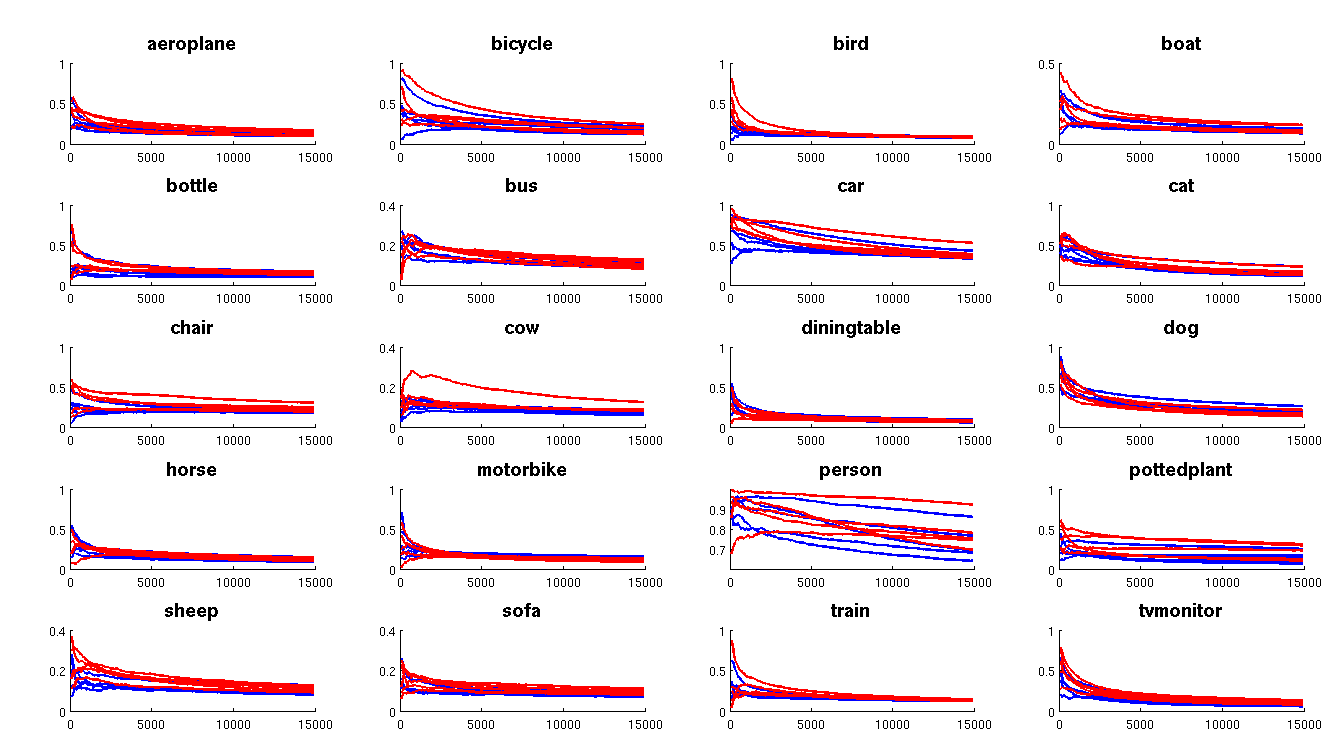
\includegraphics[scale=0.20]{images/prob_sel_dims_top5.png}
%\caption{This plot shows the precision curve for the top 5 most selective filters taken from Alex-Net (Blue) and FT-Net(Red) for all PASCAL classes. Y-axis is the precision and X-axis is number of examples.}
%\label{fig:prob-sel}
%\end{figure}

\subsection{How distributed are the feature representations?}
\label{sub:how-many}
\begin{figure}[t!]
\centering
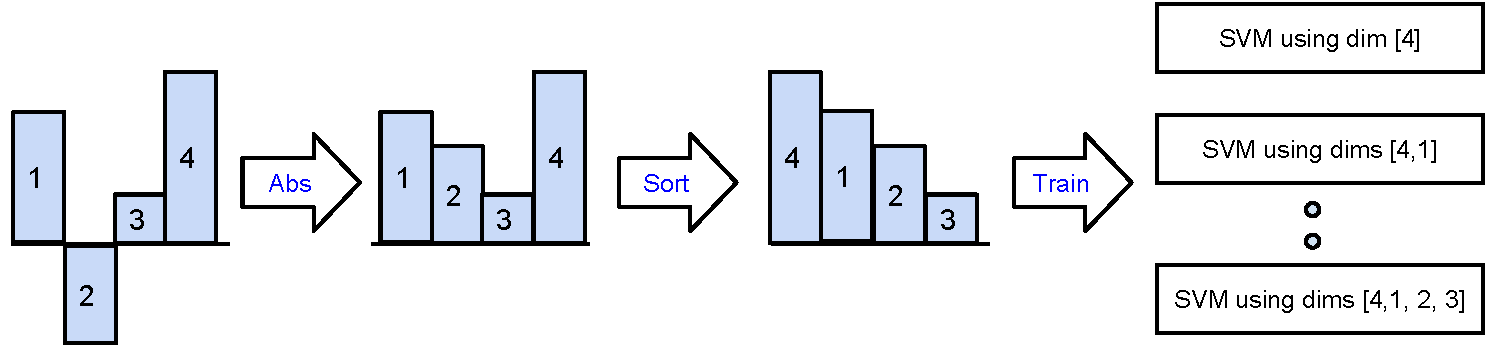
\includegraphics[scale=0.35]{images/how-many.pdf}
\caption{Illustration of the greedy strategy used for selecting filters. For each class, a linear SVM is trained after ``sp-max'' feature transformation described in section \ref{sub:imp-loc} is applied. ``sp-max''  reduces conv-5 features into a 256-D vector, wherein each dimension corresponds to one of the 256 conv-5 filters. The magnitude of individual dimensions of the weight vector learned by SVM is used as a proxy for determining the importance of each dimension. For the sake of clarity, this procedure is described using a 4-D weight vector shown on the extreme left (the numbers on each bar are the dimension). Firstly, we take the absolute value for each dimension and then sort the dimensions based on this value. Then, we chose the top k filters/dimensions from this ranked list to construct a subset of size k.}
\label{fig:sel-strategy}
\end{figure}

In addition to visualizing the AP curves of individual filters, we objectively determined the number of filters required to recognize objects of a particular class. Feature selection was performed to construct subsets \footnote{filter subsets of size [1,2,3,5,10,15,20,25,30,35,40,45,50,80,100,128,256] were used.} of consequently increasing number of filters using the greedy strategy described in figure \ref{fig:sel-strategy}. The variation in performance with the number of filters is shown in figure \ref{fig:svm-sel-dims}. 

\begin{figure}[t!]
\centering
%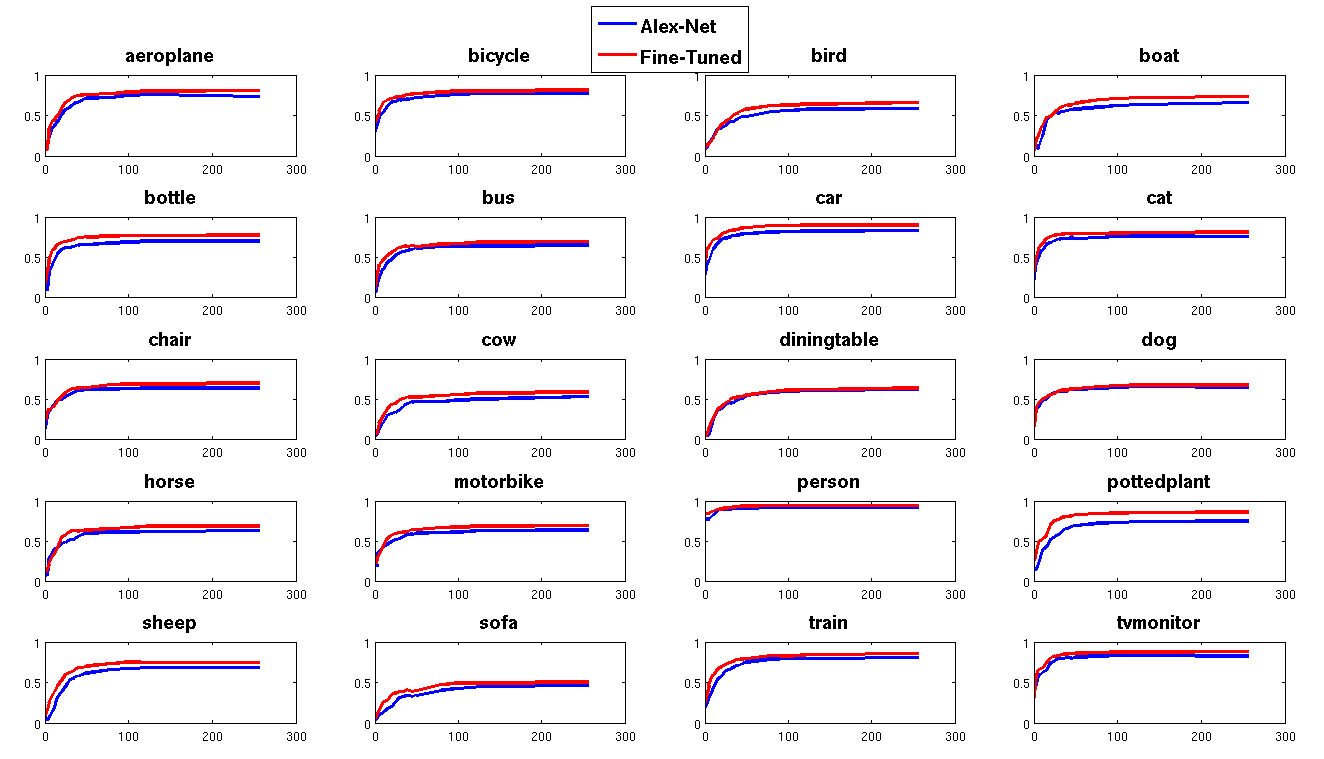
\includegraphics[height=6.5cm]{images/svm_seldims.png}
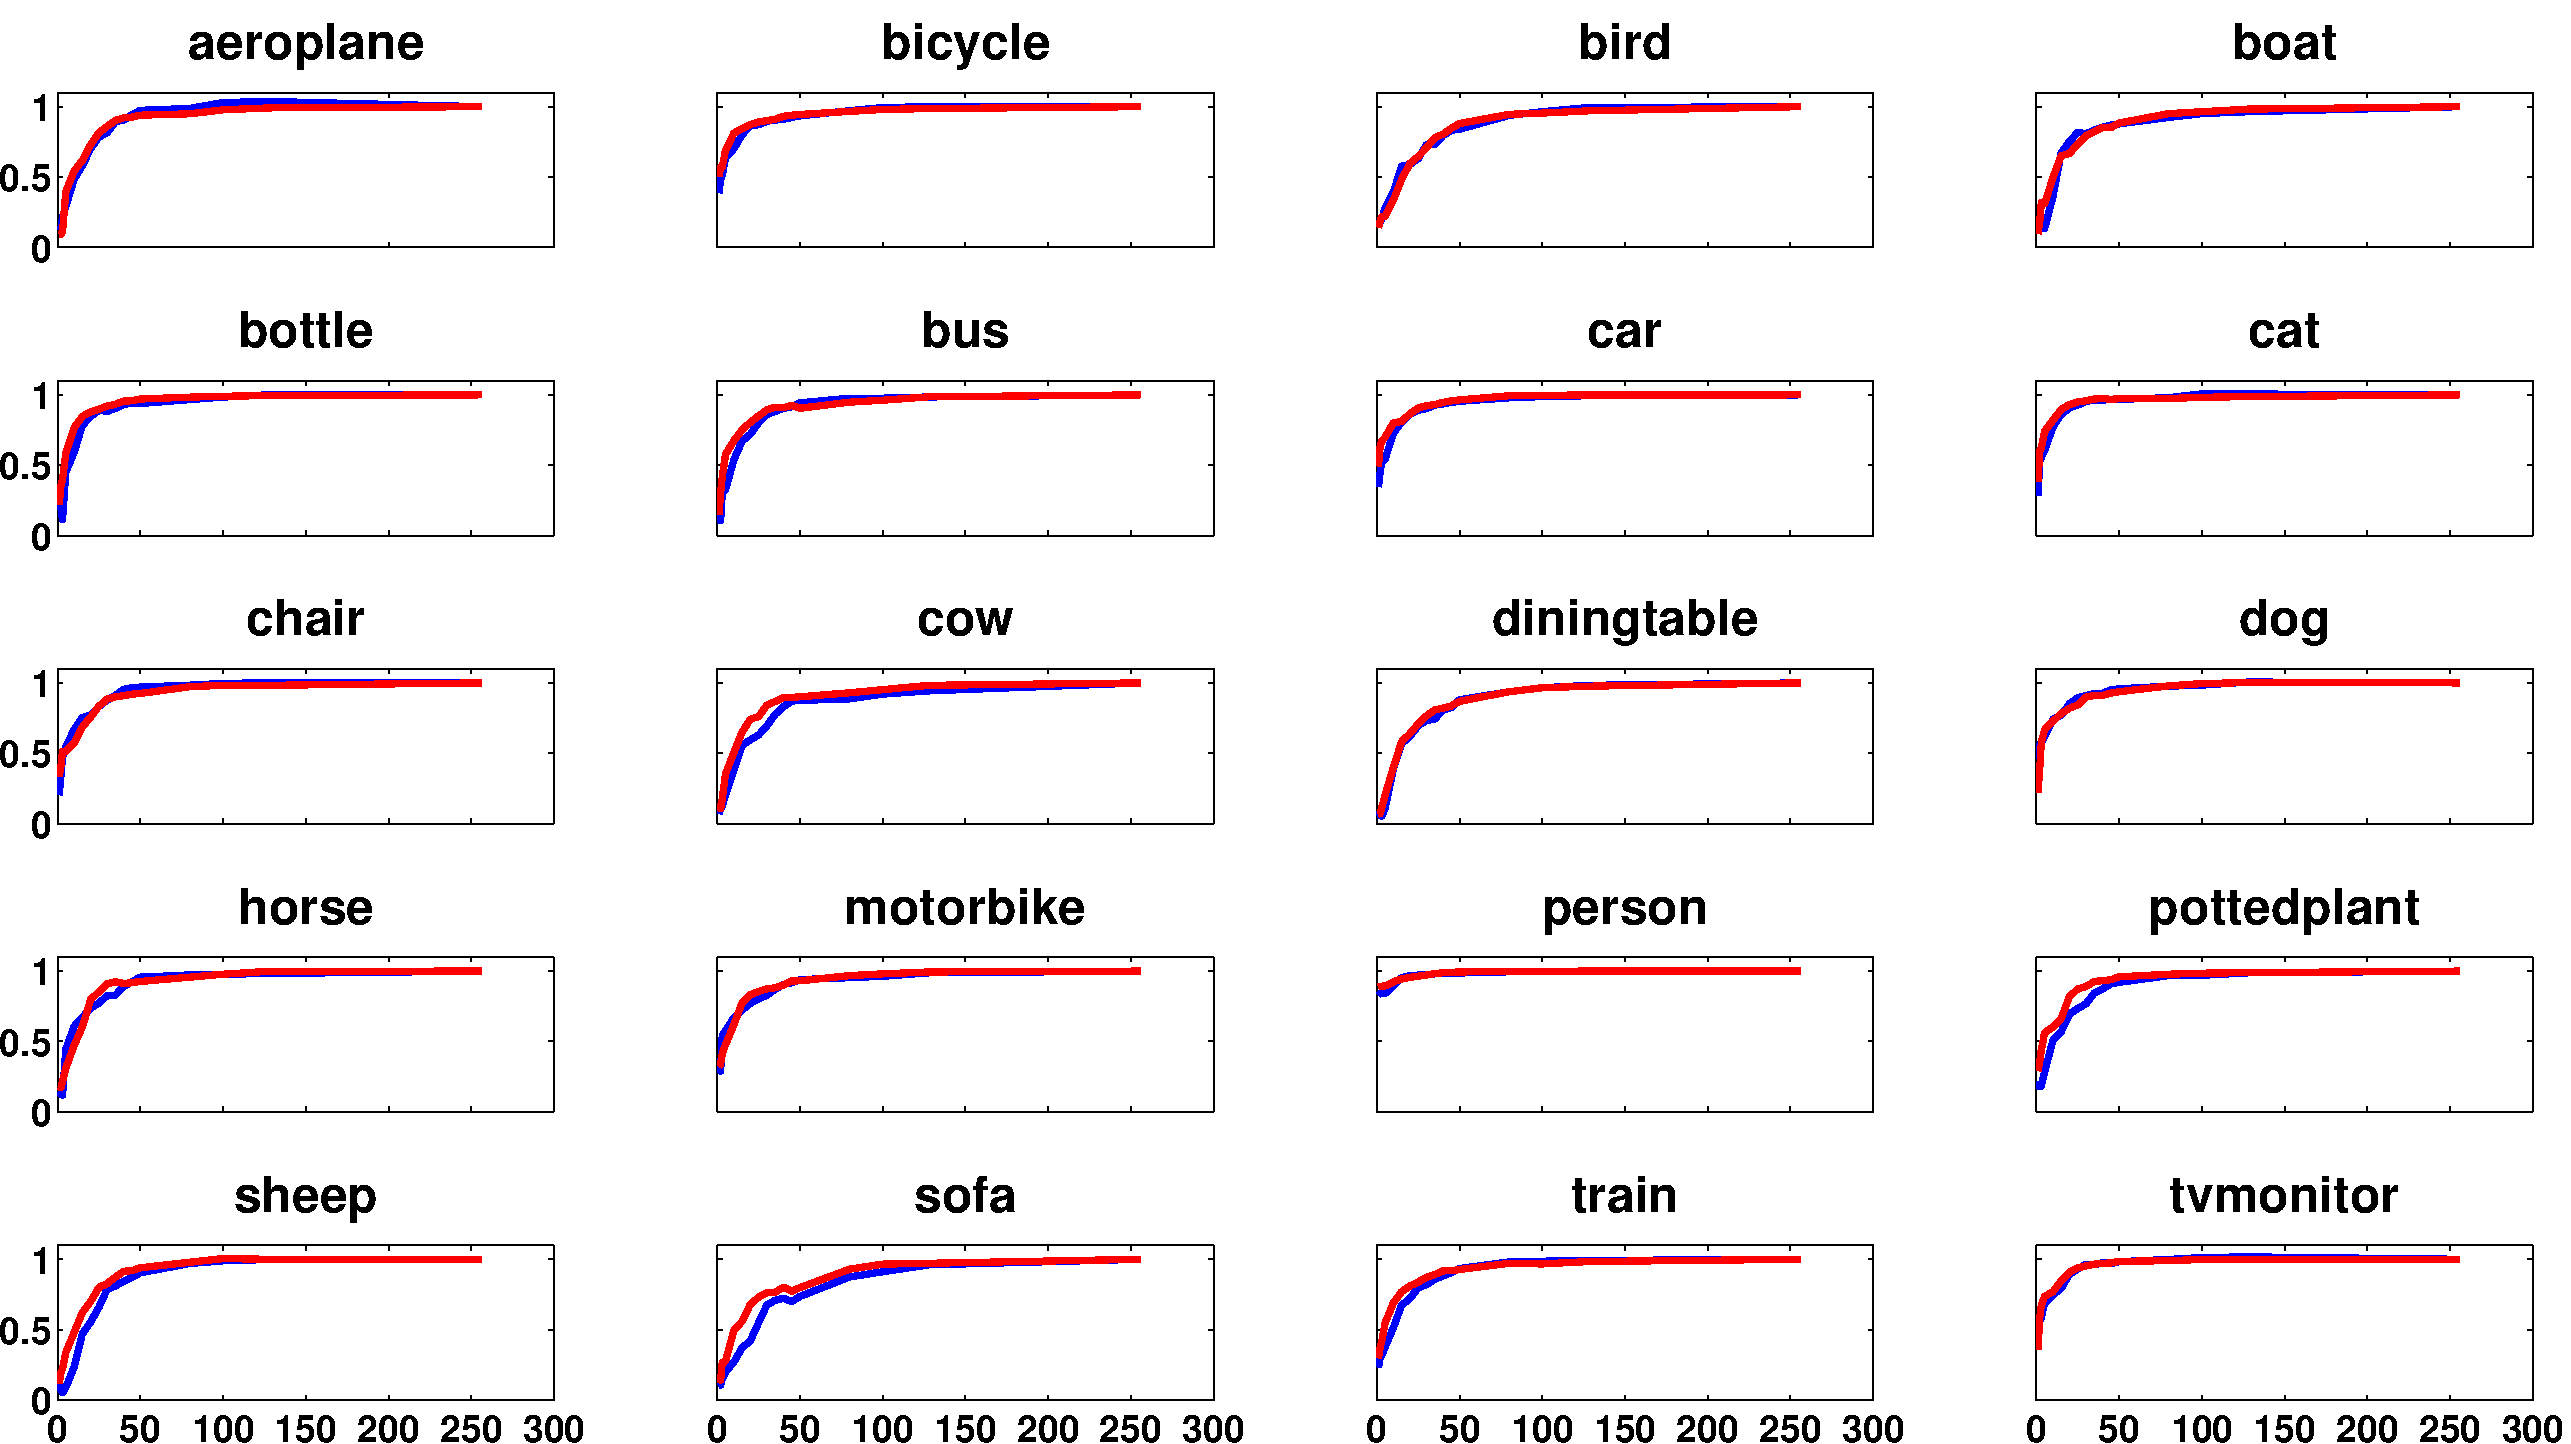
\includegraphics[height=6.5cm]{images/pool5_spmax_num_svm_filters.pdf}
\caption{ The fraction of complete performance (Y-Axis) on PASCAL-DET-GT achieved by conv-5 filter subsets of different sizes (X-axis). Complete performance is the AP computed by considering responses of all the filters. Notice, that for a few classes such as ``person'' and ``bicycle'' only a few filters are required, but for most classes substantially more number of filters are needed.}
\label{fig:svm-sel-dims}
\end{figure}  

\setlength{\tabcolsep}{1pt}
\begin{table}[t!]
\begin{center}
\caption{Number of filters required to achieve 50\% ,90\% of the complete performance on PASCAL-DET-GT using a CNN pre-trained on Imagenet and fine-tuned for PASCAL-DET using conv-5 features.}
\label{table:num-fil}
\tiny
\begin{tabular}{lc||cccccccccccccccccccc}
\hline\noalign{\smallskip}
CNN & AP & aero & bike & bird & boat & bottle & bus & car & cat & chair & cow & table & dog & horse & mbike & person & plant & sheep & sofa & train & tv \\
\noalign{\smallskip}
\hline
pre-train & 50\% & 15 & 3 & 15 & 15 & 10 & 10 & 3 & 2 & 5 & 15 & 15 & 2 & 10 & 3 & 1 & 10 & 20 & 25 & 10 & 2 \\ 
fine-tune & 50\% & 10 & 1 & 20 & 15 & 5 & 5 & 2 & 2 & 3 & 10 & 15 & 3 & 15 & 10 & 1 & 5 & 15 & 15 & 5 & 2 \\
\hline
\noalign{\smallskip}
pre-train & 90\% & 40 & 35 & 80 & 80 & 35 & 40 & 30 & 20 & 35 & 100 & 80 & 30 & 45 & 40 & 15 & 45 & 50 & 100 & 45 & 25 \\
fine-tune & 90\% & 35 & 30 & 80 & 80 & 30 & 35 & 25 & 20 & 35 & 50 & 80 & 35 & 30 & 40 & 10 & 35 & 40 & 80 & 40 & 20 \\
\hline
\end{tabular}
\end{center}
\end{table}
\setlength{\tabcolsep}{1.4pt}
  
Table \ref{table:num-fil} lists the number of filters required to achieve 50\% and 90\% of the complete performance. For classes such as persons, cars and cats a relatively few number of filters are required but for most classes around 30-40 filters are required to achieve atleast 90\% of the full performance. This indicates that in conv-5, for a few classes there are GMC like filters, but mostly the feature representation are distributed \footnote{Please see the supplementary material for results on fc-7}. We also find that after fine-tuning, slightly fewer number of filters are required to achieve performance levels similar to a pre-trained network. 

\begin{figure}[t!]
\centering
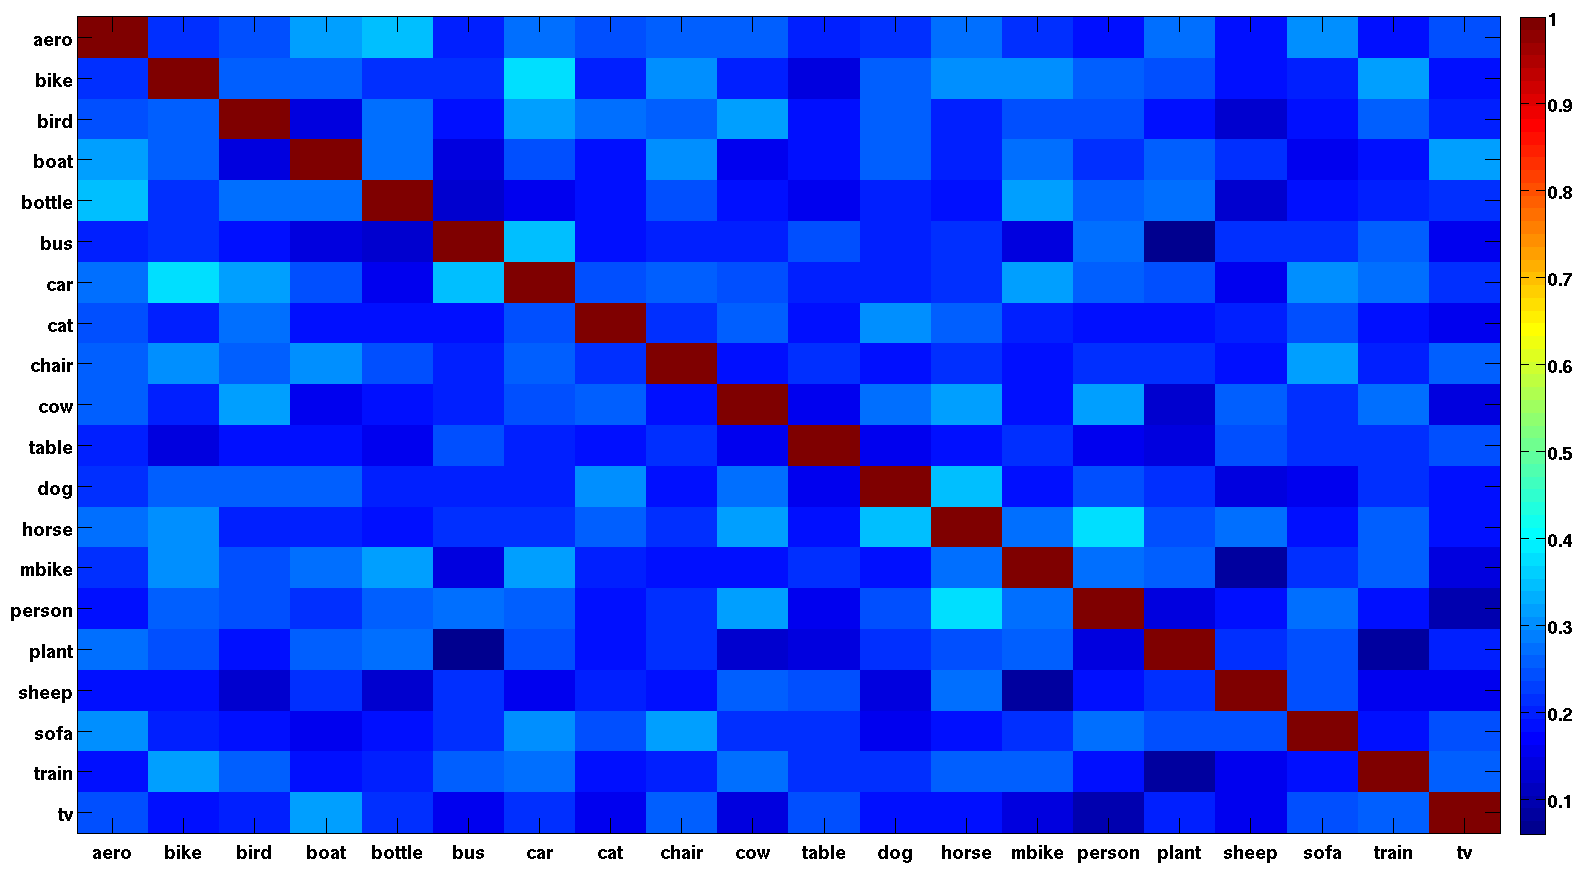
\includegraphics[width=1.0\linewidth]{images/ftNet_commonfilters.png}
\caption{The extent of overlap between the top-50 filters of conv-5 for each class determined using PASCAL-DET-GT.
Entry (i,j) of the matrix is the fraction of filters of class i common with class j (section \ref{sub:how-many}). It can be seen, that there is little overlap between filters used for different classes.}
\label{fig:overlap}
\end{figure}

Next, we estimated the extent of overlap between the filters used for discriminating different classes. Towards this end, for each class the 50 most discriminative filter were chosen. The extent of overlap was evaluated by:
\begin{align}
\frac{S_{cl^i} \cap S_{cl^j}}{N}
\end{align}
where, $S_{cl^i}$ is the set of filters for class $i$ and $N = |S_{cl^i}| = |S_{cl^j}| = 50$. The results are visualized in figure \ref{fig:overlap}. It can be seen that different classes use different subsets of conv-5 filters and there is little overlap between classes. This further indicates that intermediate representations in CNN are distributed and different sets of are used to distinguish between different classes. 

